\section{Experimental Evaluation}
\label{sec:evaluation}

In this section we are going to present the results gotten from our experimental evaluation. We start off by giving a brief overview of how we can(not) determine the complexity of a Futoshiki problem instance a priori in \Cref{subsec:futoshiki_difficulty}, we then move onto presenting the actual HW used to perform such tests in \Cref{subsec:experimental_setup}. 

We then present some common ground strategies used across every problem that we have run: Precoloring in \Cref{subsec:precoloring_performance} and Factor \Cref{subsec:factor}.

We move towards presenting our parallel solutions in \Cref{subsec:parallel_performance_analysis}, starting with MPI and OMP in \Cref{subsubsec:solving_times_mpi_omp}, we give an overview of the Speedup and Efficiency of our solution in \Cref{subsubsec:speedup_efficiency} and finally we present the results for our Hybrid implementation in \Cref{subsubsec:hybrid_results}.

We wrap up the section by performing the strong scalability analysis in \Cref{subsec:scalability}: MPI first in \Cref{subsubsec:mpi_scalability}, then OMP in \Cref{subsubsec:omp_scalability} and finally Hybrid one in \Cref{subsubsec:hybrid_scalability}.


In order to get the reader accustomed with what we are evaluating, we present only a subset of the whole family of instances that we have evaluated for this project. We specifically center our focus towards a 9x9 instance, so that the reader can understand how different solutions compare given the same problem to solve. In case you are more interested, you can find more plots in our Google Drive Folder \cite{drive}.

As we have chosen to show only a specific 9x9 in order to not let the reader get confused with the parameters under which we are showcasing our solution performs, the conclusion we are going to track are relative to this instance. As we are going to see that stating the difficulty of an instance \textit{a priori} is an hard task, findings for our 9x9 instance might not hold for another 9x9 instance. Let's say we are finding that MPI in this case outperforms the hybrid solution: this does not mean that the MPI is better \textit{overall}, but that for the specific instance considered it is better and might be worse in another instance of the problem. If we wanted to have an omni comprehensive study this would require to analyze each instance on its own, which would imply analyzing the results for each problem instance. This does not mean that the analysis is useless, instead this shall serve as a rule of thumb to showcase the capabilities when taking into account the parallelization of Futoshiki solvers. 

If the reader is interested in seeing how the solution performs under different instances, but without having a detailed analysis, he can find some extra results in the aforementioned drive folder.


\subsection{Can we evaluate difficulty of a Futoshiki before solving it?}
\label{subsec:futoshiki_difficulty}
It is important to stop for a moment and assess a crucial factor: as we have already explained in \Cref{subsubsec:backtrack} how Futoshiki has dynamic placed constraints, which in turn implies that the assumption we can make on the input are less strict w.r.t. Sudoku. This means that by receiving as input only the number of constraints, without knowing where they are placed and how they are intertwined one to another, it is extremely hard to define the actual "difficulty" of the problem. It is easy to see that with a simple manipulation of the constraints presented in \Cref{fig:futoshiki_example}, one could not have easily understood the chain between values 1-4. Another factor to take into account is where the initial numbers are placed and how many we have. It is true as the number of constraints that we have increases, the more variables we can fix and therefore the less big the search spaces becomes, but if those constraints are placed in a "bad way", one could not find the solution easily.

We can also say that the "size matters" in this case it not strictly true. One could imagine a puzzle of a specific size and one of a slightly bigger size: let's say 9x9 and 10x10. Given those as inputs, as the correlation among constraint is so important that just like for the amount of numbers placed, they might not lead to an "easier" or "harder" puzzle by default.
To wrap up this consideration, we can safely say that if we are only given number of constraints, number of initialized cells and size of the problem it is not possible to give a precise estimate over a metric to evaluate the "difficulty" of the problem.

For this reason the \textit{Weak Scalability analysis} cannot be performed in our specific case, because in order to devise the entries for which we evaluate we cannot just say 5x5, ... 9x9, 10x10 and so on, as they are not the only discriminant factor.

\subsection{Experimental Setup}
\label{subsec:experimental_setup}
We now move onto some first consideration on the underlying Hardware, to have an idea of what the numbers that we are going to see actually mean.

All experiments were conducted on a high-performance computing cluster with the following specifications:
\begin{itemize}
    \item \textbf{Hardware:} 126 nodes with Intel Xeon processors.
    \item \textbf{Network:} 10Gb/s Ethernet with Infiniband/Omnipath options.
    \item \textbf{Software:} Linux CentOS 7, GCC 9.1, MPICH 3.2.
    \item \textbf{Test Cases:} Various puzzles from 5×5 to 11×11, including "hard" instances.
\end{itemize}

\subsection{Impact of Pre-coloring Optimization}
\label{subsec:precoloring_performance}
As we have already discussed in \Cref{subsubsec:precoloring}, the precoloring procedure helps us at doing some pre computation, which in turn lets us reduce the search space of our solution. In \Cref{fig:precoloring_improvement} we see how by performing precoloring gives us better results w.r.t. the standard brute force approach. In the X axis we have 3 different 9x9 problems to be solved, and in the Y axis the total time measured in seconds for \textit{the solving time of our algorithm only}.

\begin{figure}[htbp]
\centering
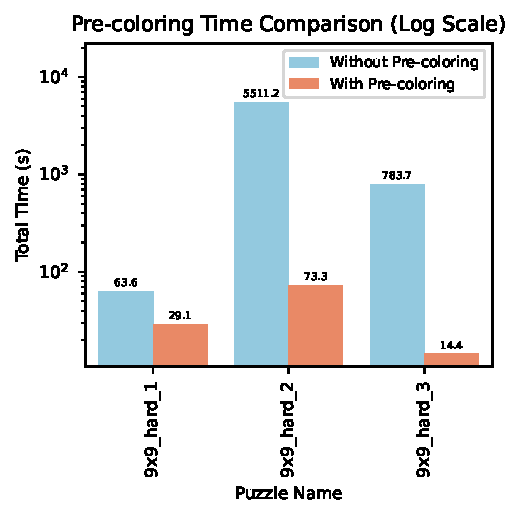
\includegraphics[width=0.9\linewidth]{imgs/precoloring_comparison.pdf}
\caption{Comparison of execution times for some 9x9 futoshiki problems}
\label{fig:precoloring_improvement}
\end{figure}


This figure lets us understand that by employing this technique we can see up to 54x speedup, like in the case of the instance \textit{9x9\_hard\_3}. This means that even if we have a little bit of overhead to apply the list coloring solution, we can still see great improvements over the baseline. For this reason we chose to employ precoloring on all of the following case studies, so that we both reduce the amount of variables in our comparison while introducing several fold speedup in our proposed solution.

\subsection{What the factor are we talking about?}
\label{subsec:factor}
We have already mentioned that our solutions have a parameter presented as \textit{Configurable Factor}. We said that this factor lets us tweak the ratio between the jobs being scheduled and the underlying computational unit (either a thread for the OpenMP case, or a CPU for the MPI one). From an high level point of view we can think it as a knob that lets us choose at our will the amount of "pressure" that we are putting the underlying system in.

From a more formal point of view, given a factor F and the number of underlying computational units C, our preprocessing algorithm aims at going deeper and deeper into the search space by exploring the backtrack tree until it does not find an amount of puzzles to solve P such that:
\[
    F * C \leq P
\]

This lets us play around to find the best possible ratio, which therefore lets us find the maximum amount of "stress" to put our computational units at before we have generated too many jobs for them.

In fact, we have run several tests to assess which factor could be the best one to choose from, so we now present our \textit{Factor Analysis} that we have devised to pick it.


\begin{figure}[htbp]
\centering
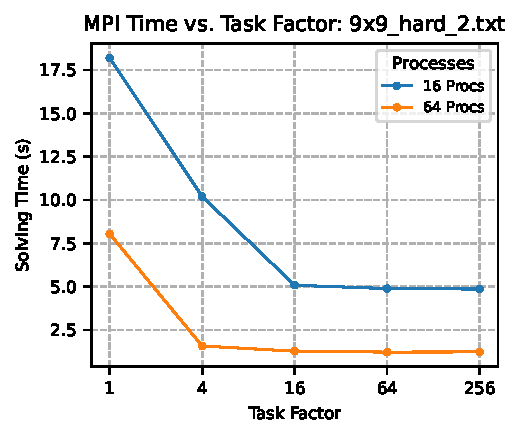
\includegraphics[width=0.9\linewidth]{imgs/factor_mpi_9x9_hard_2.pdf}
\caption{factor analysis for MPI}
\label{fig:factor_analysis_mpi}
\end{figure}

\begin{figure}[htbp]
\centering
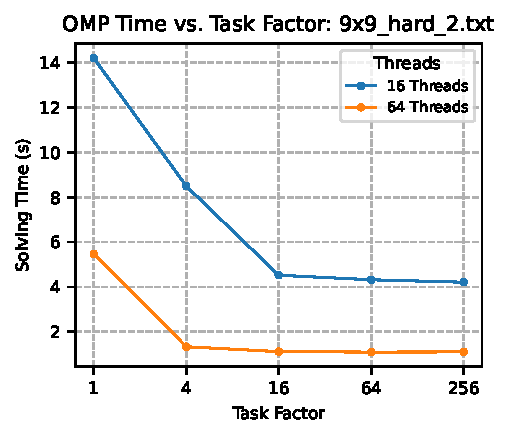
\includegraphics[width=0.9\linewidth]{imgs/factor_omp_9x9_hard_2.pdf}
\caption{factor analysis for OMP}
\label{fig:factor_analysis_omp}
\end{figure}

\begin{figure}[htbp]
\centering
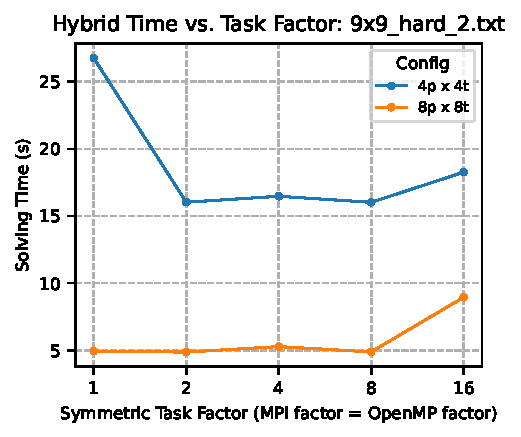
\includegraphics[width=0.9\linewidth]{imgs/factor_hybrid_9x9_hard_2.pdf}
\caption{factor analysis for hybrid solution}
\label{fig:factor_analysis_hybrid}
\end{figure}

From \Cref{fig:factor_analysis_mpi} and \Cref{fig:factor_analysis_omp} we can see that we have a good slope in the decreasing of the solving time of our solution with 16 processors/threads up until 64, and then we start to stabilize. 

After running other experiments, we have seen that 64 was most of the times the elbow point at which we would see diminishing returns and for this reason we picked such value.

As for the hybrid, we have faced the issue on "how can we evaluate MPI and OMP solutions"? In order to provide some interesting results, we have decided to abstract away from the actual implementation of the worker (MPI or OMP), and we have therefore decided to treat a processor in MPI as the same as the threads for OMP. This modeling simplification is going to help us in \Cref{subsubsec:hybrid_results} when evaluating how the hybrid solution works under several different configurations.

After having taken this necessary detour, we can move towards finding the best factor for the hybrid one: we can see from \Cref{fig:factor_analysis_hybrid} that if we consider the symmetric factor 8, which means setting MPI Factor to 8 and Openmp Factor to 8, if we take this approximation into account (considering processors = threads), we can see how 8*8=64 is also a fairly good factor in this case.


For this reason, we have decided to set for the following runs MPI and OMP factor to 64, and for the hybrid the MPI Factor to 8 and its symmetric counterpart to 8, so that we would have a factor of 64 "computational units" across the board.


The concept of oversubscription, it being creating more tasks than workers is well-established in parallel computing, and as we have seen with a factor of 64 we can see up to \textbf{3.5x}.

\subsection{Parallel Performance Analysis}
\label{subsec:parallel_performance_analysis}

After having understood how hard it is to evaluate the difficulty of our problem \textit{a priori}, and having set the ground for our base configuration (hardware used, pre coloring algorithm, factor selected), we can finally move into the evaluation of how our parallel solutions work.

\subsubsection{Solving times for MPI and OMP}
\label{subsubsec:solving_times_mpi_omp}

We start off by showing how our MPI and OMP solutions work with a 9x9\_hard instance and a 10x10\_hard instance (note that the "hard" concept comes from how the website from which we have taken the problems from ranked them. Here are the 2 main sources which we downloaded from \cite{puzzle_futoshiki,puddelbee} and converted images to compatible representation via a custom parser which we have devised in order to gather data).

Please note that as the cluster has a maximum amount of thread per node set to 64, we cannot gather data in the case of 128 threads due to HW constraints. This is the main reason why in the following plots there is not going to be an entry for OMP with 128 Computational units.


We start off by showing a 9x9 instance in \Cref{fig:comparison_solving_time_9x9}. On the x axis we have the number of computational units that we are using, and on the Y axis the time it required for our algorithms to find a valid permutation of numbers to solve the puzzle.

We can see that, as we expect, as the number of computational units increase, the solving time for our problem decreases as we can extract more and more parallel work.

The red dotted line serves as a baseline, as it is the time required for our sequential algorithm to find a solution and it is going to be present in the next graphs also, so that one can easily understand how a given parallel implementation compares w.r.t. the sequential one. Please note that, as also the execution of the sequential algorithm is depending on the hardware, what we are presenting is an average over the execution times of the sequential solution.


We can see that for 1 and 2 we have values which are in the range of the sequential algorithm minus some seconds of delta in the measurement and this is because, as we have already presented in the \Cref{sec:solution} we have decided to opt for the sequential algorithm to remove the overhead given by OMP and MPI.

\begin{figure}[htbp]
\centering
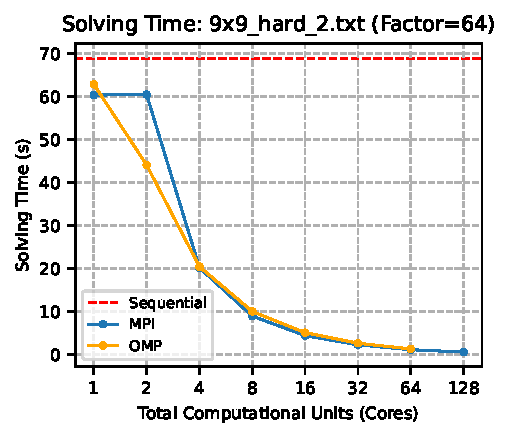
\includegraphics[width=0.9\linewidth]{imgs/solving_time_mpi_omp_9x9_hard_2.pdf}
\caption{Solving time comparison for a 9x9 instance}
\label{fig:comparison_solving_time_9x9}
\end{figure}

We now move towards a 10x10 instance. In \Cref{fig:comparison_solving_time_10x10} we see something strange: every parallel implementation is consistently worse w.r.t. solving time compared to the sequential solution (minus some cases like the 4,8 and 16 CU which have little to no actual increase in performance). 

This is very interesting, because by looking at the absolute value of the solving time we can note that even the sequential algorithm is taking less than 0.01 second to find the solution. This lets us draw two necessary conclusions:
\begin{enumerate}
    \item As we have stated in \Cref{subsec:futoshiki_difficulty}, the size alone is not a factor which directly implies the difficulty of the problem. We can see that the absolute time to solve the 9x9 and 10x10 are vastly different, even if someone might at a first glance say "if we have more cells we should have higher execution times". This does not always hold if we do not consider all of the aforementioned variables.
    \item Parallel solutions introduce some overhead, either the message passing infrastructure needed for the MPI framework to process messages, or the locks needed to achieve high efficiency shared memory reading and writing when accessing critical parts of code. Such overhead is usually mitigated by the fact that the overall \textit{speedup} in finding a solution is higher than the overhead introduced by parallelizing the work. This is not the case for these specific families of problems: as the sequential solution is already extremely fast, it does not make sense to parallelize it, and therefore we can conclude that this family of instances are not tailored or our parallel solution analysis.
\end{enumerate}

For such reasons, we are going to move to analyze only the family of 9x9 instances, as they are more interesting and actually give us some interesting data and points to reason about w.r.t. just saying "for the 10x10 instance we have a degradation in performance".

We have decided to insert an image of the Futoshiki problem taken into consideration, which is the 9x9\_hard\_2 and it can be seen in \Cref{fig:9x9_img}

\begin{figure}[htbp]
\centering
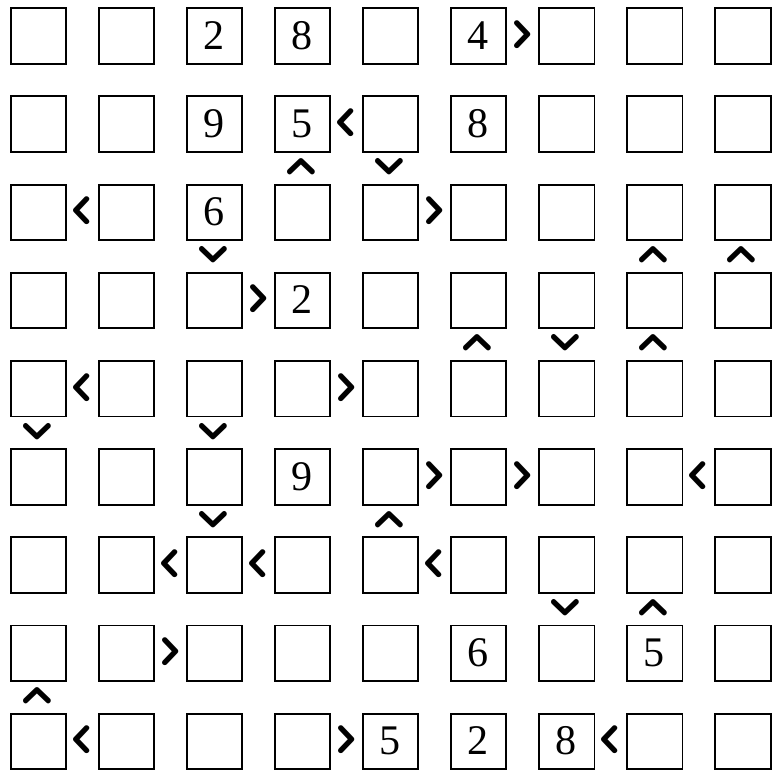
\includegraphics[width=0.9\linewidth]{imgs/9x9_hard_2_puzzle.png}
\caption{Our problem instance taken into consideration for evaluation purposes.}
\label{fig:9x9_img}
\end{figure}

\begin{figure}[htbp]
\centering
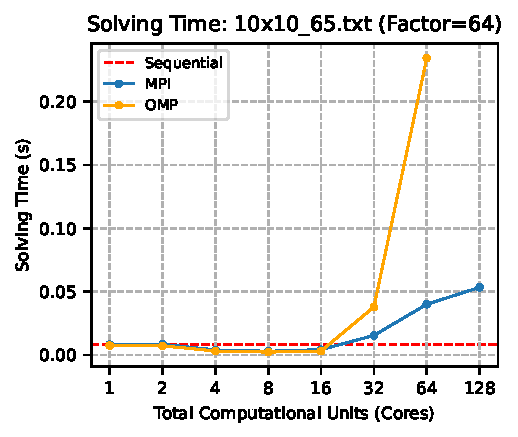
\includegraphics[width=0.9\linewidth]{imgs/solving_time_mpi_omp_10x10_65.pdf}
\caption{Solving time comparison for a 10x10 instance}
\label{fig:comparison_solving_time_10x10}
\end{figure}

\subsubsection{How well does parallel solution perform compared to sequential?}
\label{subsubsec:speedup_efficiency}

Now that the reader has understood how configurations and difficulty of the puzzles impact the overall execution time, he might ask himself "is there a metric to evaluate how much better the parallel solutions are compared to the sequential one?"

Turns out that we have such metrics. We know that if we have a task and we parallelize it, we can use the \textit{Speedup} concept to understand how much better it gets, and it is presented as:
\[
S = \frac{Execution\_time\_sequential}{Execution\_time\_parallel}
\]
This means that the lower the execution time is when parallelized, the higher the speedup is going to be. In \Cref{fig:speedup_9x9} we show the speedup that we can reach with our solution. On the x axis w.h. the computational units, whereas in the Y axis we have the speedup value. The red line represents the theoretical speedup that we can reach, so assuming that the parallelization of the task introduces absolutely 0 overhead.


We can see that, while for MPI the speedup is close to the ideal one, for the OMP case it is not. Of course, again, we do not have the 128 computational unit present for OMP as we are capped at 64 threads.

We can also conclude something interesting:
\begin{enumerate}
    \item As the number of computational units increase, we introduce higher overhead due to the message passing or the shared variables accesses, which is not much if we have "few" computational units, but as the number goes up the overhead is getting a little bit bigger, therefore impacting the overall speedup. For this reason we see that the theoretical line and the real one strand further and further as the number of the CU increase.
    \item Another kind of overhead to consider is the one introduced by \textit{Resource Contention}, which is happening due to increasing the amount of threads and cpus utilizing the same memory, therefore reducing the effective memory bandwidth or saturating caches.
    \item The fact that the speedup does not grow as fast as the ideal one does not mean that the solution gets slower: It is still faster than the sequential solution.
\end{enumerate}


\begin{figure}[htbp]
\centering
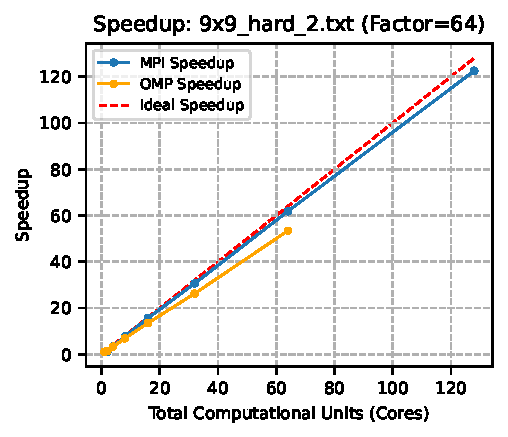
\includegraphics[width=0.9\linewidth]{imgs/speedup_mpi_omp_9x9_hard_2.pdf}
\caption{Speedup of parallel solutions}
\label{fig:speedup_9x9}
\end{figure}

We can now move into the second metric that we can use to evaluate our parallel algorithm w.r.t. the sequential one: the \textit{Efficiency}. This is a derivative parameter which is dependent on the speedup, and it can be expressed as:
\[
E = \frac{Speedup}{\# computational\_units}
\]

This parameter is basically relating the speedup (how well the parallel solution is w.r.t. the sequential one) with the number of units available. This parameter is therefore going to tell us how well the available cores are being used.

\Cref{fig:efficiency_9x9} we can see how efficiency is evaluated in our solutions. 

We can make some considerations here:
\begin{enumerate}
    \item MPI is strictly dominating the OMP efficiency plot, and this tells us that MPI overhead due to the shared memory access is higher than the message passing approach used by MPI, which is fairly interesting.
    \item We see a degradation in efficiency for MPi with 2 CUs. This is due to the fact that for MPI with 2 workers we are basically running the sequential under the hood: 1 master and 1 slave with the MPI message passing overhead, so it is perfectly expected.
\end{enumerate}

\begin{figure}[htbp]
\centering
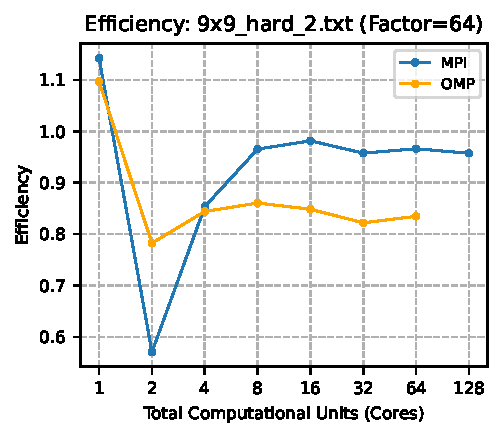
\includegraphics[width=0.9\linewidth]{imgs/efficiency_mpi_omp_9x9_hard_2.pdf}
\caption{Efficiency of parallel solutions}
\label{fig:efficiency_9x9}
\end{figure}


\subsubsection{How does the Hybrid solution perform?}
\label{subsubsec:hybrid_results}

Now that we have presented the MPI and OMP solution we can move to our hybrid solution. For this one we have devised 3 scenarios: one in which we would balance the number of CPU for MPI and threads for OMP, one in which we relied more on the MPI rather than OMP and the latter one viceversa. 

This means that if we have for example 16 available computational units, we would have the balanced setting with 4 cpus for MPI and 4 threads for each MPI slave, whereas for the other cases we would have 2 cpus and 8 threads or 8 cpus and 2 threads respectively. 

Note that we have already fixed the factor to 8 and 8 in \Cref{fig:factor_analysis_hybrid}, which is not to be confused with the available CPUS/Threads that we are selecting.

The main reason is to assess if for the tasks given and the architecture of our solution, it would be better to rely more on MPI or OMP -- or maybe a balanced approach would be the best...

This is what we are trying to answer with \Cref{fig:solving_time_hybrid_9x9}. We present the same instance of 9x9 which we are evaluating the parallel solutions in order to have less variables to consider. The structure is the same: we have the red line representing the average solving time for our sequential time and we color coded the balanced, MPI Heavy and OMP Heavy accordingly. Over the Y axis the solving time measured in seconds.

We can take several notes:
\begin{itemize}
    \item As expected, as the number of CU increase the solving time reduces.
    \item The sweet spot to get a performance increase lies in the 8-32 zone and after that for the law of diminishing returns we can see that actually we are not improving by a lot in terms of absolute values.
    \item we can see how actually the choice of relying on one or another one does not influence too much the overall execution time if the number of units increase, no matter whether they are threads or cpus.
    \item We can see an outlier with MPI Heavy and 2 Computational units. This is due to the fact that we are running the sequential solution under the hood with the overhead of message passing from MPI.
\end{itemize}

\begin{figure}[htbp]
\centering
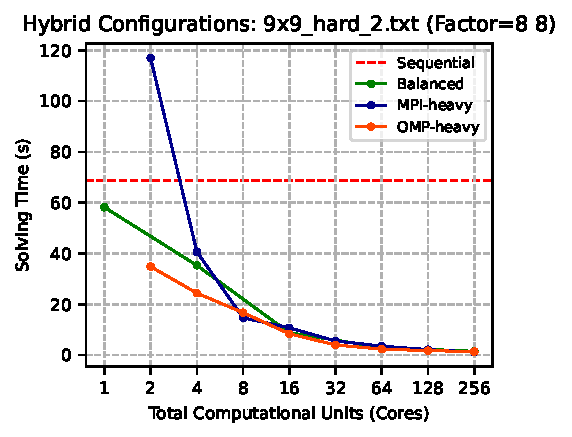
\includegraphics[width=0.9\linewidth]{imgs/solving_time_hybrid_9x9_hard_2.pdf}
\caption{Solving time for hybrid solution}
\label{fig:solving_time_hybrid_9x9}
\end{figure}

We can now move onto the comparison among hybrid and sequential, just like we did for the normal solutions: we start off with the Speedup in \Cref{fig:speedup_hybrid}.

Also here we can draw some conclusions:
\begin{itemize}
    \item The overall speedup is not as close as the ideal one just like for the MPI and OMP only cases. This is actually expected, as we have seen how the overhead added from the underlying technology (locks to access shared memory in OMP, waiting algorithms used in MPI solution to sync messages) actually add an overhead, and the more computational units we have, the more they compound.
    \item We can see that up to 128 computational units the OMP heavy solution has a little bit more of an advantage compares to the other ones, but at 256 the MPI heavy solution surpasses the other ones (which can also mean, it does not degrade as much as the other ones).
\end{itemize}


\begin{figure}[htbp]
\centering
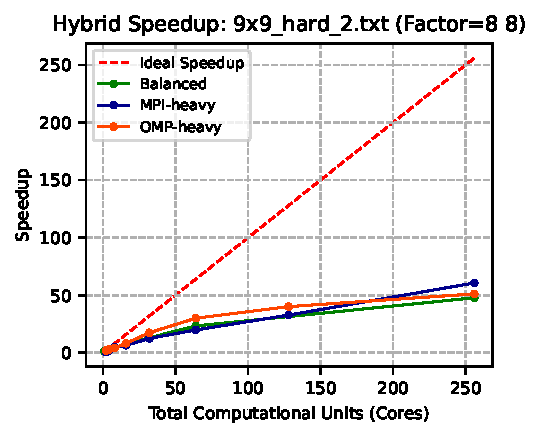
\includegraphics[width=0.9\linewidth]{imgs/speedup_hybrid_9x9_hard_2.pdf}
\caption{Speedup of hybrid solution}
\label{fig:speedup_hybrid}
\end{figure}


We now move onto the last metric, it being the \textit{Efficiency}. From \Cref{fig:efficiency_hybrid} we can see that:
\begin{itemize}
    \item The overall efficiency is less compared to the standard MPI and OMP only approaches, and this is due to the aforementioned overhead from the underlying technologies used.
    \item There is a strict trend in this case: as the number of computational units increase, the overall efficiency decreases. This is expected as the more Computational units we have, the less each one is contributing towards the final result w.r.t the solving time. It would be interesting to play around with the factor to overload more the computational units to see how the efficiency performs.
    \item As the efficiency value is basically a mirror over the speedup, as we have seen that the speedup was not on the same level as the speedup for the classic solutions, we were actually expecting that the efficiency would decline as the computational units increase.
\end{itemize}


\begin{figure}[htbp]
\centering
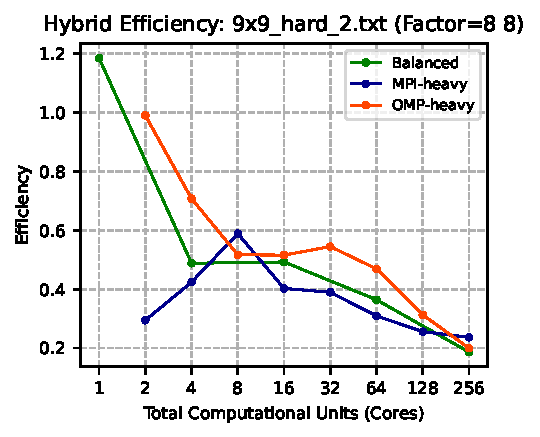
\includegraphics[width=0.9\linewidth]{imgs/efficiency_hybrid_9x9_hard_2.pdf}
\caption{Efficiency of hybrid solution}
\label{fig:efficiency_hybrid}
\end{figure}

\subsection{Strong Scalability: MPI, OMP and Hybrid}
\label{subsec:scalability}

In this subsection we are going to show our strong scalability analysis given MPI, OMP and Hybrid solutions. These are going to be presented in a tabular fashion to give an easier way of seeing absolute values compared to the trends that we have already seen up until now with the plots.

\subsubsection{MPI Scalability}
\label{subsubsec:mpi_scalability}
Table \ref{tab:mpi_scaling} presents MPI performance across multiple nodes:

\begin{table}[htbp]
\caption{MPI Strong Scaling (9×9 Hard Puzzle)}
\begin{center}
\begin{tabular}{@{}cccc@{}}
\toprule
\textbf{Processes} & \textbf{Time (s)} & \textbf{Speedup} & \textbf{Efficiency} \\
\midrule
1   & 60.27 & 1.00   & 100.0\% \\
2   & 60.37 & 1.14   & 57.0\% \\
4   & 20.17 & 3.41   & 85.4\% \\
8   & 8.92  & 7.72   & 96.5\% \\
16  & 4.38  & 15.70  & 98.2\% \\
32  & 2.25  & 30.64  & 95.8\% \\
64  & 1.11  & 61.82  & 96.6\% \\
128 & 0.56  & 122.54 & 95.7\% \\
\bottomrule
\end{tabular}
\end{center}
\label{tab:mpi_scaling}
\end{table}


MPI shows a "quasi linear" scaling in speedup terms. We see how with 1 and 2 the execution time is practically the same (minus noise given by underlying hardware, scheduling of resources, etc), but then it quickly reduces. We can see how the overall efficiency values are higher than OMP, suggesting that MPI is better suited to stress the underlying hardware, which is exactly what we have seen in \Cref{fig:efficiency_9x9}.

\subsubsection{OpenMP Scalability}
\label{subsubsec:omp_scalability}
Table \ref{tab:omp_scaling} shows OpenMP performance with increasing thread counts on a single node:

\begin{table}[htbp]
\caption{OpenMP Strong Scaling (9×9 Hard Puzzle)}
\begin{center}
\begin{tabular}{@{}cccc@{}}
\toprule
\textbf{Threads} & \textbf{Time (s)} & \textbf{Speedup} & \textbf{Efficiency} \\
\midrule
1  & 62.78 & 1.00  & 100.0\% \\
2  & 44.01 & 1.56  & 78.2\% \\
4  & 20.40 & 3.38  & 84.4\% \\
8  & 10.00 & 6.88  & 86.0\% \\
16 & 5.07  & 13.57 & 84.8\% \\
32 & 2.62  & 26.30 & 82.2\% \\
64 & 1.29  & 53.41 & 83.5\% \\
\bottomrule
\end{tabular}
\end{center}
\label{tab:omp_scaling}
\end{table}

The OMP solution shows a good improvement as the number of thread increase. Up until 16 threads the solving time almost halves each time. It is worth noting that the efficiency remains extremely high also for 64 threads, which means that the solution holds very well on shared memory systems.


\subsubsection{Hybrid Scalability}
\label{subsubsec:hybrid_scalability}
The hybrid solver demonstrates superior scalability by combining both paradigms:

\begin{table}[htbp]
\caption{Hybrid Scaling (9×9 Hard Puzzle)}
\begin{center}
\begin{tabular}{@{}ccccc@{}}
\toprule
\textbf{Processes} & \textbf{Threads} & \textbf{Time (s)} & \textbf{Speedup} & \textbf{Efficiency} \\
\midrule
1  & 1  & 58.17 & 1.00  & 100.0\% \\
1  & 2  & 34.81 & 1.98  & 98.9\% \\
1  & 4  & 24.35 & 2.83  & 70.7\% \\
2  & 2  & 35.29 & 1.95  & 48.8\% \\
2  & 4  & 16.66 & 4.13  & 51.7\% \\
2  & 8  & 8.35  & 8.25  & 51.6\% \\
4  & 1  & 40.62 & 1.70  & 42.4\% \\
4  & 2  & 14.63 & 4.71  & 58.9\% \\
4  & 4  & 8.74  & 7.88  & 49.2\% \\
4  & 8  & 3.95  & 17.42 & 54.4\% \\
4  & 16 & 2.29  & 30.01 & 46.9\% \\
8  & 2  & 10.69 & 6.44  & 40.3\% \\
8  & 4  & 5.52  & 12.47 & 39.0\% \\
8  & 8  & 2.95  & 23.30 & 36.4\% \\
8  & 16 & 1.72  & 40.09 & 31.3\% \\
8  & 32 & 1.35  & 51.15 & 20.0\% \\
16 & 4  & 3.48  & 19.80 & 30.9\% \\
16 & 8  & 2.10  & 32.76 & 25.6\% \\
16 & 16 & 1.44  & 47.77 & 18.7\% \\
32 & 8  & 1.14  & 60.63 & 23.7\% \\
\bottomrule
\end{tabular}
\end{center}
\label{tab:hybrid_scaling}
\end{table}


Here we presented the hybrid solution by increasing first the threads. We can see how the efficiency overall reduces due to the MPI and OMP overhead, which means that the synchronization overhead basically compounds as the number of computational units increase. Overall this table shows how we can still achieve high performances increase, but at the cost of a worse efficiency, which would suggests us that the best setting if we want to maximize this metric is the MPI solution.
